%-----------------------------------------------------------
\chapter{\hatterismeret}\label{chap:hatter}
%-----------------------------------------------------------

\section{Modellezés}
\subsection{Modell-alapú rendszerfejlesztés}
A modell-alapú rendszerfejsztés, angolul rövidítve MBSE\footnote{Model-based systems engineering}, egy formalizált módszertan, amely a követelméynkezelés, tervezés, analízis, verifikáció és validáció témaköreiben nyújt segítséget az összetett rendszerek fejlesztése során.
A dokumentum-alapú fejlesztéssel ellentétben az MBSE modelleket helyez a fejlesztés középpontjába.
A 2020-as évben a NASA\footnote{National Aeronautics and Space Administration, Amerikai Egyesült Államok kormányzati ügynöksége} is megjegyezte, hogy ,,A modell-alapú rendszertervezést mind az ipari mind a kormányzati egyre inkább felkarolja, hogy lépést tudjon tartani a rendszer komplexitásával.''\cite{Nasa2020}
Az MBSE három különböző koncepciót hoz össze: modell, rendszergondolkodás, rendszerfejlesztés (Shevchenko, 2020 \cite{shevchenko_2020})

A modell-alapú rendszerfejlesztés növelheti az a teljes termék specifikációhoz tartozó információ megragadásának, vizsgálatának, megosztásának és koordinálásának képességét, amely a következő előnyökkel járhat (Friedenthal, 2007 \cite{friedenthal2007incose}):
\begin{itemize}
    \item Javítja a kommunikációt a fejlesztésben részvevők között (például: a vevő, a projekt vezető, a rendszermérnökök, hardver és szoftver fejlesztők, tesztelők stb.).
    \item Az összetettség menedzselésének javítása.
    \item Megnövekedett termék minőség.
    \item A rendszertervezés alapjainak tanítási és tanulási képességének javulása.
\end{itemize}

Manapság a modell-alapú rendszertervezés számos iparágban jelen van, például: Járműipar, közlekedés, űripar, orvosi eszközök, robotika, nukleáris technológia, ipari rendszrek, gyártás stb.
Leginkább olyan környezetekben használatos, ahol valóság korlátos (beavatkozás behatárolt, méret kényszer stb.), 
fontos az együttműködés több szakmán/beszállítókon keresztül, 
drága a prototípus gyártás vagy biztonságkritikus rendszereknél (Molnár, 2019 \cite{rete0}).

\subsection{SysML}
A SysML\footnote{Systems Modeling Language} egy általános célú architektúra modellező nyelv rendszermérnöki felhasználásra.
A nyelv támogja számos rendszerek, rendszerek rendszereinek (Systems of systems) specifikálását, vizsgálatát, tervezését, verifikációját és validációját.
Ezek tartalmazhatnak hardver/szoftver elemeket, információkat, folyamatokat, személyzetet és létesítményeket.
A SysML az UML\footnote{Unified Modeling Language} 2-nek egy dialektusa és egy UML 2 Profilként van definiálva \cite{sysml}.

A SysML Cris Kobryn által szervezett rendszermérnökökből és modellező eszköz szakértőkből álló informális szövettség úgy nevezett ,,SysML Partnekek'' által lett létrehozva 2003-ban.
Az első kiadás 2005-ben jelent meg és az elsődleges közreműködök között ott volt a Motorola, a Telelogic és a Northrop Grumman is.
Másfél évvel az első megjelenés után, 2006-ban hivatalosan is adaptálásra került a specifikáció az OMG\footnote{Object Management Group} által, ezáltal a specifikáció hivatalos neve: OMG SysML 1.0.
A mai napig nem történt nagy változás a szabványban. A jelenleg használt legfrissebb verzió az 1.5-ös, bár az OMG 2017-ben benyújtott egy változtatást OMG SysML 2.0 néven \cite{sysml-partner}.

\subsubsection{Modell elemek}
Mint az már fentebb említve lett, a SysML kiegészíti az UML 2 nyelvet.
A két nyelv kapcsolatát az \ref{fig:sysUML}. ábra szemlélteti.
Látható, hogy egyes elemek teljesen kikerültek a SysML eszközkészletéből, de számos újdonság került bele.

\begin{figure}
    \footnotesize
    \centering
    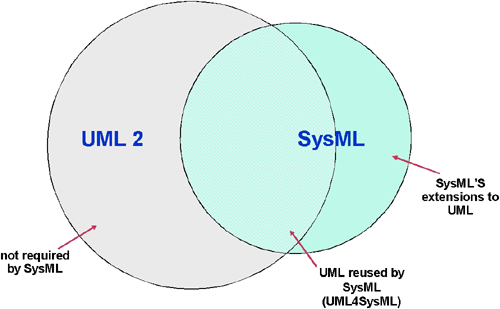
\includegraphics[width=100mm, keepaspectratio]{figures/sysml_uml.jpg}
    \caption{A SysML és az UML kapcsolata (Forrás: \cite{omgsysml})}
    \label{fig:sysUML}
\end{figure}

A SysML struktúrájának alapvető egysége a blokk, amit bármilyen rendszer elem reprezentálására lehet használni (például: hardver, szoftver, létesítmény, személyzet stb.).
A rendszerstruktúrát blokk definíciós diagrammok (BDD\footnote{Block Definition Diagram}) és ,,internal block'' diagrammok (IBD\footnote{internal block diagram}) alkotják.
A BDD írja le a rendszer hierarhiáját, míg az IDB a belső struktúrát.

A nyelv támogat számos viselkedésleíró diagrammot is. Ezek nagyrésze egyezik az UML-ben definiált párjával.
Az egyetlen kivétel az Aktivitás diagramm, amely kissé módosult az adaptáció során.

A hasonlóságokat és különbségeket legjobban az \ref{fig:sysDiag}. ábra mutatja be.

\begin{figure}
    \footnotesize
    \centering
    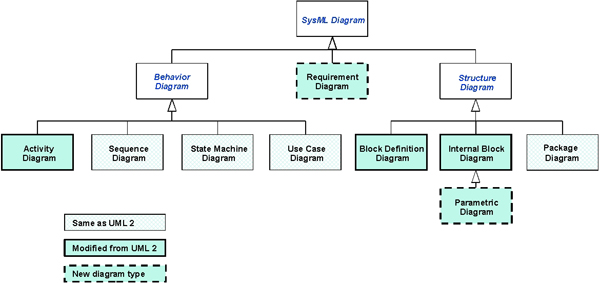
\includegraphics[width=100mm, keepaspectratio]{figures/sysml_diagrams.jpg}
    \caption{SysML diagramm típusok (Forrás: \cite{omgsysml})}
    \label{fig:sysDiag}
\end{figure}